\chapter[The SSID Protocol]{The Soundscape Indices (SSID) Protocol: A Method for Urban Soundscape Surveys -- Questionnaires with Acoustical and Contextual Information}

%TODO: Still need to fix tables
%TODO: Edit intro / add context of this being a stand-alone scientific work.

Conducting urban soundscape studies on a scale large enough to form a machine learning dataset presents a unique challenge. The standardised methods of conducting soundscape surveys \citep{ISO12913_2_2018IOS} are labour-intensive, time-consuming, and provide limited information about the acoustical and environmental context.

\section*{Abstract}

 A protocol for characterizing urban soundscapes for use in the design of \gls{ssid} and general urban research as implemented under the European Research Council (ERC)-funded SSID project is described in detail. The protocol consists of two stages: (1) a Recording Stage to collect audio-visual recordings for further analysis and for use in laboratory experiments, and (2) a Questionnaire Stage to collect in-situ soundscape assessments via a questionnaire method paired with acoustic data collection. Key adjustments and improvements have been made to enable the collation of data gathered from research groups around the world. The data collected under this protocol will form a large-scale, international soundscape database.

\section{Introduction}
 %NOTE: This intro might work better to form the thesis intro. Then jump into the protocol at "Purpose" and design

 %NOTE: Could replace with an intro which ends up justifying the development of the protocol as its own stand-alone scientific work.

 Soundscape studies strive to understand the perception of a sound environment, in context, including acoustic, (non-acoustic) environmental, contextual, and persona factors. These factors combine together to form a person's soundscape in complex interacting ways \cit{1}. In order to predict how people would perceive an acoustic environment, it is essential to identify the underlying acoustic and non-acoustic properties of soundscape.

 The soundscape community is undergoing a period of increased methodological standardisation in order to better coordinate and communicate the findings of the field. This process has resulted in many operational tools designed to assess and understand how sound environments are perceived and apply this to shape modern noise control engineering approaches. Important topics which have been identified throughout this process are soundscape 'descriptors', 'indicators', and 'indices'. \citet{Aletta2016Soundscape} defined soundscape descriptors as "measures of how people perceive the acoustic environment"; soundscape indicators as "measures used to predict the value of a soundscape descriptor"; and soundscape indices can then be defined as "single value scales derived from either descriptors or indicators that allow for comparison across soundscapes" \citep{Aletta2018Towards}.

 This conception has recently been formalised and expanded upon with the adoption of the recent ISO 12913 standard series \citep{ISO12913_1_2014IOS,ISO12913_2_2018IOS,ISO12913_3_2019IOS}. ISO 12913 Part 1 sets out the definition and conception of Soundscape, defining it as the "acoustic environment as perceived or experienced and / or understood by a person or people, in context". Here, the soundscape is separated from the idea of an acoustic environment, which encompasses all of the sound which is experienced by the receiver, including any acoustically modifying effects of the environment. In contrast, the soundscape considers the acoustic environment, but also considers the impact of non-acoustic elements, such as the listener's context and the visual setting, and how these interact with the acoustic environment to influence the listener's perception.

 The ISO/TS 12913-2:2018 is the current reference document addressing data collection and reporting requirements in soundscape studies. In terms of methods, the ISO document covers two main approaches, namely: soundwalks combined with questionnaires (Methods A and B) and narrative interviews (Method C) \citep{ISO12913_2_2018IOS}, which relate to on-site and off-site data collection, accordingly. Part 3 of the ISO 12913 series builds on Part 2 and provides guidelines for analysing data gathered using only those methods \citep{ISO12913_3_2019IOS}. However, the range of possible methodological approaches to soundscape data collection is much broader and it includes, for instance, laboratory experiments \citep{Aletta2016Soundscape,Sun2019Classification,Oberman2018Towards}, pseudo-randomized experience sampling \citep{Craig2017Experience}, and even non-participatory studies \citep{Lavia2018Non}. The protocol described in this paper was designed having in mind the need for a relatively large soundscape dataset that could be used for design and modelling purposes, thus trying to expand the scope of soundwalks that typically deal with much smaller samples of participants \citep{Engel2018Review}. For the sake of comparability and standardization with these methods, we chose to refer to the soundscape attributes reported in the ISO Part 2 (Method A).

 Several studies prior to the formalisation of the ISO standards on soundscape demonstrated the general, but inadequate, relationship between traditional acoustic metrics, such as $L_{Aeq}$, with the subjective evaluation of the soundscape \cit{1, 12-15}. These have typically aimed to address the existing gap between traditional environmental acoustics metrics and the experience of the sound environment. \citep{Yang2005Acoustic} showed that, when the sound level is 'lower than a certain value, say 70 dB(A)', there is no longer a significant change in the evaluation of acoustic comfort as the sound level changes. However, the perceived sound level does continue to change along with the measured sound level, showing that (1) measured sound level is not enough to predict soundscape descriptors such as 'acoustic comfort', and (2) there is a complex relationship between perceived sound level and soundscape descriptors which is mediated by other factors.

 % NOTE I've written this intro section in a few places. I'm going to move on to the protocol specific stuff and decide what to do with the above later.

\section{Purpose}

 The \gls{ssid} Protocol was designed to achieve two primary goals:
 \begin{enumerate}
   \item gather in-situ soundscape assessments from the public, which can be further analysed and utilised in designing a soundscape index;
   \item conduct recordings needed to reproduce the audio-visual environment of a location in a laboratory setting for conducting controlled experiments on soundscape.
 \end{enumerate}

 These two goals represent two levels of data required for developing a general soundscape model. The first enables large scale data collection, resulting in a database with thousands of perceptual responses and their corresponding quantitative data which can be statistically analysed on a large scale, or used for training in machine learning modelling. In-situ assessments also represent the most holistic assessment, ensuring all factors that influence the soundscape are present, including those which cannot be reproduced elsewhere.

 However, there are questions that cannot be practically addressed in-situ, such as soundscape assessment of less- or un-populated areas, the influence of mismatched acoustic and visual cues, physiological and neural responses to various soundscapes, and so on \cit{31}. Laboratory experiments with controlled environments are required to address these aspects. Toward the development of a coherent \gls{ssid}, therefore, it is important that these two forms of data are collected simultaneously and with compatible methods, such that the results of the two approaches can be confidently combined and compared. In addition, since this protocol is intended to be used for the creation of a large-scale international database with additions carried out by several different and remote teams, it has been designed for efficiency, scalability, and information redundancy.

\section{Protocol Design and Equipment}
 The first goal is achieved by conducting in-situ questionnaires using a slightly altered version of Method A (questionnaire) from Annex C of the ISO/TS 12913-2:2018 technical specification \citep{ISO12913_2_2018IOS} collected either via handheld tablets or paper copies of the questionnaire. Typically, a minimum of 100 responses are collected at each location during multiple 2-5 hr sessions over several days. During the survey sessions, acoustic data are collected via a stationary class 1 or class 2 \gls{slm} (as defined in IEC 61672-1:2013 \cit{IEC61672}) running throughout the survey period and through binaural recordings taken next to each respondent. These acoustic and response data are linked through an indexing system so that features of the acoustic environment can be correlated with individual responses or with the overall assessment of the soundscape, as required by researchers.

 The second goal is achieved by making First-Order (or higher) Ambisonic recordings simultaneously with 360\degree video which can be reproduced in a virtual reality environment. It has been shown that head-tracked binaural and multi-speaker ambisonic reproduction of recorded acoustic environments recorded in this way have high ecological validity \cit{33}, particularly when paired with simultaneous head-tracked virtual reality video \cit{22, 34, 35}.

 The on-site procedure to collect these data are separated into two stages, which will be outlined in detail in Section \ref{sec:proc}. The stage during which the audio-visual recordings are made for lab experiments is called the \textbf{Recording Stage}, while the stage during which questionnaires and environmental data are captured is called the \textbf{Questionnaire Stage}.

 The procedure has been designed to include multiple levels of data and metadata redundancy, making it robust to on-site issues and human error. The most crucial aspect of the redundancy is ensuring the perceptual responses can be matched with the appropriate corresponding environmental and acoustic data even when some information is lost or forgotten.

 \subsection{Labelling and Data Organisation}
   \label{section:metadata}
   In order to be able to identify all of the many data components of the Recording and Questionnaire Stages and to associate these with their various corresponding data, the following labelling system is suggested. This system is focussed on (1) relating all of the separate recordings and factors to specific questionnaire responses and (2) efficiency and consistency on site. A recent paper by \citet{Aumond2017Modeling} demonstrated the importance of addressing multiple levels of factors which influence perception, from individual-, to session-, to location-level. The successful pleasantness models built incorporating these information levels showed a marked improvement over the equivalent individual-level or location-level only models. The data organisation system proposed here was designed in order to maintain this important information, and the levels of information for the data collected on site are shown in Table \ref{tab:metadata}.

   At the top level is the \textbf{Location} information. This includes information about the location which does not change day-to-day, and generally characterises the architectural character of the space, or typical climate conditions for the area. As described in Section \ref{sec:loc-selection}, each '\gls{environmental-unit}' should be considered a new location. Therefore, if researchers want to investigate the differences in soundscape assessment in the middle of a small urban park and along the road next to the same park, these would be considered different locations since they would (typically) have different environmental factors and should be given difference names. The name chosen should be concise, but it should be obvious what location is referred to.

   The next level is information which is specific to each session, labelled with a \textbf{SessionID}. This SessionID should contain the name of the location and a numerical index which will increase with each repeated session at that location. The SessionID is associated with the data collected during the Recording Stage, and with the data which are continuous throughout the Questionnaire Stage, SLM, and ENV data. For easy automatic processing, correct spelling and consistency with the format is crucial so that data can be filtered according to the SessionID or the location, as is often necessary. In addition, for ease of automatic processing, it is recommended not to include spaces in the SessionID to avoid string splitting issues in analysis code.

   Underneath each SessionID will be a set of \textbf{GroupID}s. One GroupID is assigned for \emph{each group of participants}. This should correspond to a single binaural recording and a single 360\degree photo. This will be used to (1) relate multiple surveys taken simultaneously and (2) link the recording and photo with the surveys. The GroupID is particularly crucial as it allows commonly missing data to be shared across multiple collection methods. For instance, occasionally paper questionnaires will be missing start and end time information. In this case, this information can be pulled directly from other questionnaires with the same GroupID. Where no questionnaires have the times, it is possible to extract an approximate start time from the binaural recordings or 360\degree photo and then estimate an average end time.

   The GroupID should have the following format: [a set of letters representing the location name][the SessionID index number][an incrementing index for each group]. For example, for the second session at Regent's Park Japanese Garden, the location name is 'RegentsParkJapan', the GroupID letters might be 'RPJ'; the SessionID would be 'RegentsParkJapan2', so the GroupIDs for that session would start at '201'. Therefore, for example, the tenth group of participants for that session would be labelled 'RPJ210'. This format ensures that, if the location or SessionID are not recorded for a questionnaire, it is still obvious which session it belongs to.

   % Please add the following required packages to your document preamble:
   % \usepackage{booktabs}
   % \usepackage{graphicx}
   \begin{table}[]
     \centering
     \resizebox{\textwidth}{!}{%
       \begin{tabular}{@{}cclccccc@{}}
         \toprule
         \textbf{Level of information} & \multicolumn{6}{c}{\textbf{Example Label}} & \textbf{Factors measured at this level}                                                                                                                             \\ \midrule
         Location                      & \multicolumn{6}{c}{RegentsParkJapan}       & GPS, Architectural typology, visual openness, etc.                                                                                                                  \\ \midrule
         SessionID                     & \multicolumn{4}{|c|}{RegentsParkJapan1}    & \multicolumn{2}{c|}{RegentsParkJapan2}             & SLM, session notes, ENV                                                                                        \\ \midrule
         GroupID                       & \multicolumn{2}{|c|}{RPJ101}               & \multicolumn{1}{c|}{RPJ102}                        & \multicolumn{1}{c|}{...} & \multicolumn{1}{|c|}{RPJ201} & \multicolumn{1}{c|}{\ldots} & BIN, PIC               \\ \midrule
         Questionnaire                 & \multicolumn{2}{|c|}{1, 2, 3}              & \multicolumn{1}{c|}{4, 5}                          & \multicolumn{1}{c|}{...} & \multicolumn{1}{c|}{25, 26}  & \multicolumn{1}{c|}{\ldots} & QUE, Start \& End time \\ \bottomrule
       \end{tabular}%
     }
     \caption{Labelling system for on site data collection. Regents Park Japanese Garden is used as an example location. Abbreviations as defined in Table \ref{table:factors} - SLM: Sound Level Meter (acoustical factors); ENV: Environmental factors; QUE: Questionnaires; PIC: Site pictures.}
     \label{tab:metadata}
   \end{table}

   %%%%%%%%%%%%%%%%%%%%%%%%%%%%%%%%%%%%%%%%%%%%%%%%%%%%%%%%%%%%%%%%%%%%%%%%%%%%%%%%%%

 \subsection{Location and Measurement Point Selection}
   \label{sec:location-selection}

   To select the appropriate measurement point, it should be ensured that the following contextual factors representative of the site are present in the spatial recording: openness, greenness, presence of landmarks, dominant use (walking, staying), and social presence (related to the dominant use). These are identified as objective metrics often used in urban and landscape research \cit{36-40}, possibly contributing to soundscape assessment \cit{23, 41}. This relies on the researcher's opinion-drive assessment -- it is advised to observe the location for a moment and then choose the point representative of the context and the first-person user experience. For instance, in a park, it would probably be near a bench in the central area near the fountain; in a busy square, it would be a place where most people gather and have the best view of the landmark. While doing so, the placement too near the prominent vertical objects such as a statue, a wall, or a mast should be avoided as it might cause issues in later handling the visual data (3m is considered a safe distance from these features). Similar concerns are also true for the audio data and careful attention should be paid to avoid placing the recording equipment near extraneous noisy equipment or acoustic shadows. Further guidance on this is given in Point 4 of Section \ref{sec:proc}. It is important to avoid placing the recording equipment at a position where no users are expected (i.e. don't put the equipment in the middle of a flower bed or a grass area that nobody uses).

   For the purposes of this protocol, a single location was considered to be an '\gls{environmental-unit}' wherein the environmental factors are consistent and is typically perceived to constitute a single distinct area. The exact dimensions and delineation of the \gls{environmental-unit} will vary depending on the characteristics of the space, so it is ultimately up to the judgement of the researchers on site to select an appropriate measurement point to best capture the character of the \gls{environmental-unit}.

 \subsection{Equipment}
   \label{sec:equipment}
   %TODO: Check table referencing issues
   The equipment listed in Table \ref{tab:equipment} is designed to facilitate both the audio-visual recording of the location and the collection of objective environmental factors, as given in Table \ref{tab:factors}. What equipment is brought on site should be adjusted depending on availability, needs of the researchers, and whether only one of the protocol stages will be carried out, or both. The equipment selected should be neutral and not noticeable. In general, this means dark or neutral colours as opposed to high-visibility colours and selecting compact equipment.

   The use of class 1 or class 2 \gls{slm}s has been stipulated to maintain verifiable consistency and quality of data across all soundscape studies which make use of this protocol, as well as with data collected under various other environmental acoustics purposes. As the accuracy of acoustic information gathered at the site is the most vital in the discussion of soundscape indices, specific requirements have only been set out for the acoustic equipment. Class 1 is highly preferred, but consideration is made for cost and availability of equipment. It should be noted what standard of \gls{slm} was used in the data collection and appropriate consideration of the precision and tolerances of the equipment should be taken during the data analysis.

   \begin{table}
     \label{tab:equipment}
     \caption{Recommended equipment for implementing the \gls{ssid} protocol. \gls{slm}: Sound Level Meter; \gls{amb}: Ambisonics; \gls{bin}: Binaural; \gls{que}: Questionnaires}

   \end{table}

   \begin{table}
     \label{tab:factors}
     \caption{Table of recommended context and acoustic measurement factors.}
   \end{table}

   %%%%%%%%%%%%%%%%%%%%%%%%%%%%%%%%%%%%%%%%%%%%%%%%%%%%%%%%%%%%%%%%%%%%%%%%%%%%%

\section{Techniques for Field Data Collection}

 There are several methods available for characterising the physical environment and collecting soundscape assessments. Here, we will address the techniques employed in this protocol and general best practice for each of them.

 \subsection{Questionnaire Surveys}

   As stated above, the questionnaire is primarily based on Method A of ISO/TS 12913-2:2018. This method begins with a set of questions relating to the sound environment which are assess on a 5-point Likert scale, coded from 1 to 5. A sample codebook to demonstrate the recommended variable naming and response coding is included in \draft{Appendix X}.
   %TODO: Fix internal references

   The first section includes four questions relating to sound source identification, where the sound sources are divided into four categories: Traffic noise, Other noise, Sounds from human beings, and Natural sounds (labelled SSI01 through SSI04, respectively). These taxonomic categories of environmental sounds are based on the work done by \citet{Guastavino2005Ecological} and \citet{Brown2018study} \cit{45}.

   Next are the 8 scales which make up the circumplex model of the \gls{ssqp} \citep{Axelsson2012Swedish}, describing the \gls{paq}. These are assessed on a 5-point Likert scale from 'Strongly Disagree (1)' to 'Strongly Agree (5)'. These are included as follows: Pleasant, Chaotic, Vibrant, Uneventful, Calm, Annoying, Eventful, and Monotonous (labelled PAQ01 through PAQ08, respectively).

   Following this are five questions addressing the participant's overall assessment of the surrounding sound environment, addressing overall acoustic quality, the appropriateness of the sound environment to the location, perceived loudness, and how often the participant visits the place and how often they would like to visit again (labelled SSS01 through SSS05, respectively).

   The fourth section comprises the \gls{who5}, asking how the participants have been feeling over the last two weeks, such as 'I have felt calm and relaxed'. The \gls{who5} index is constructed to constitute an integrated scale in which the items add up related information about the level of the individual's general psychological well-being \cit{47, 48}. This information can provide additional insight into how exposure to pleasant or annoying soundscapes may impact psychological well-being as was investigated by \citet{Aletta2019Associations} \cit{27} or, alternatively, how a person's current psychological status may influence their perception of the sound environment as recently investigated by \citet{Erfanian2021Psychological}. Each of the five \gls{who5} questions (labelled WHO01 to WHO05) are assessed on a 6-point scale coded from 0 to 5.


   The final section of the participant-facing questionnaire comprises five questions on the participant's demographic information (age [AGE00], gender [GEN00], occupational status [OCC00], education level [EDU00], ethnicity [ETH00], and local vs. tourist [MISC03]) and a free response for the participant to provide any additional comments they would like to make on the sound environment [MISC01]. It is important to note that the section on ethnicity, and to a lesser extent education level, will need to be adjusted to ensure the available responses are appropriate for the location where the survey is being conducted.

   At the end of the questionnaire are a set of spaces available for the researcher conducting the survey to fill out, adding additional information about the observed behaviour of the participants, indexing and labelling metadata, and space for any additional notes. More information and guidance on this information is included below.


   This questionnaire is intended to collect a consistent core set of perceptual responses and information about the participant, with space to add additional questions as required by specific research goals. Some examples of this have been implemented by the various research groups are specific questions calling attention to water sounds and features, the perception of visual features, and an open response for identifying the dominant sound source. Given the proper labelling and coding, these additional questions can be fully integrated into the overall dataset, allowing the researchers the freedom to pursue their own research interests while maintaining consistency and compatibility with the overall database.

   General notes for conducting the questionnaires:

   \begin{itemize}
     \item The core questionnaire is reported in \draft{Appendix C}. The labels and corresponding scales are also reported. Ideally, the form should be submitted and filled on a tablet via a survey app (e.g. REDCap, Qualtrics, KoBoToolbox, or similar) so that data can then be easily downloaded in an .xlsx or .csv file. Using paper forms is also acceptable; however, researchers on site will need to take more careful note of information such as the time of response and the information will need to be manually input after the session is completed. If using an electronic version, the system should be set up to record the start and end times and GPS coordinates for each survey.
     \item If using an electronic version, be sure to have enough tablets with internet connectivity (if required by the survey system) and sufficient battery life; if using the paper version, be sure to print enough copies. Even if using the electronic version, it is recommended to also print a number of paper versions as a backup or if a large group agrees to participate at once.
     \item Regardless of the translation of the items, it is important that the label (e.g. SSI01) is kept, as well as the size and direction of the scales (1-5, etc.) to maintain data consistency.
   \end{itemize}



 \subsection{Contextual and Environmental Factor Data Collection}

   During each survey, the equipment listed in Section \ref{sec:equipment} is set up to capture the contextual and environmental data for the location. Table \ref{tab:factors} lists the factors to be collected and at what stage they should be collected.

   \subsubsection{Spatial Audio-Visual Recordings}

   In order to capture the acoustic and visual information in the space for replication in a laboratory setting, 360\degree video and \gls{amb} audio are recording to be used in \gls{vr} playback. The goal of this is two-fold: first, to enable researchers to document and replicate the in-situ environment of the space as it was during a questionnaire survey session for lab experiments and, second, to capture environments in which performing a questionnaire survey is not feasible.

   Typically, questionnaire surveys are carried out over a period of several days at the same location. The goal of these multiple sessions is to capture as many questionnaire responses as needed (100 for a particular soundscape is typically recommended \cit{11}), which, in the experience of the authors %NOTE: May need to change pronouns, etc.
   is prohibitively difficult to achieve in a single session in most locations. It is recommended that the repeated sessions are conducted under similar circumstances and environmental conditions. As such, it is not entirely necessary to repeat the spatial recordings each time a questionnaire survey is conducted. Instead, it may be useful to use the spatial recording as a chance to gain a different perspective on the space under investigation. For instance, if the questionnaires are conducted in the middle of a large urban park, the first session could collect a spatial recording within the \gls{environmental-unit} of the questionnaire site, but the subsequent returns to the site could collect spatial recordings in a different \gls{environmental-unit}, say, along a road bounding the park, or in a space in the park which does not typically have many people. This enables the simultaneous expansion of the questionnaire database and the gathering of additional environments to investigate in a laboratory setting.

   General notes for spatial recordings:

   \begin{itemize}
     \item The audio-video recordings can be done before or after the questionnaire survey.
     \item The purpose of the audio-video recordings is to capture representative recordings which can be reproduced in a laboratory setting. During the first time at a location, the focus should on capturing the environment as experienced by the respondents to the questionnaires at that location. Therefore, the recordings should be performed in nearly the same spot, with similar lighting and environmental conditions. For further survey sessions, provided the conditions are similar, other recordings could be taken which provide additional perspectives around the space for reproducing in the lab.
     \item These recordings can be performed entirely separately from the questionnaire survey, ,if desired. Reasons for doing this may be (but are not limited to): location is not populated, making questionnaires impossible; specific locations or conditions are required for a lab experiment; time limitations require many sites in an area to be captured and in-situ questionnaires could not be completed in time.
     \item The 360\degree video will take a significant amount of storage space. Researchers should ensure that there is ample free space on the camera SD cards prior to going out on site. If conducting multiple surveys away from their home institute (i.e. in another city), teams are recommended to bring a large external hard drive so that videos can be offloaded after each session.
   \end{itemize}

   \subsubsection{Reference Recordings}

   A soundscape index, or any investigation of the impact of the physical environment on the soundscape, requires consistent and accurate measurement of the environment, most importantly calibrated measurement and recording of the acoustic environment. For this protocol, this has been achieved through the use of separate calibrated binaural recordings and measurements made with a calibrated \gls{slm}.


   %%%%%%%%%%%%%%%%%%%%%%%%%%%%%%%%%%%%%%%%%%%%%%%%%%%%%%%%%%%%%%%%%%%%%%%%%%%%%%%%%%%%%%%%

\section{Procedure}
 \label{sec:proc}

 Figure \ref{fig:timeline} shows the whole process of the on site soundscape protocol. The relevant equipment in each row should be operating when the row is coloured in, such that when multiple rows are shaded this means that multiple pieces of equipment should be running during that time period. The following section prepares step-by-step instructions for conducting the in-situ surveys, including the Recording Stage and Questionnaire Stage. Figure \ref{fig:survey-pic} shows an example of the recommended equipment setup.

 \begin{figure}
   \centering
   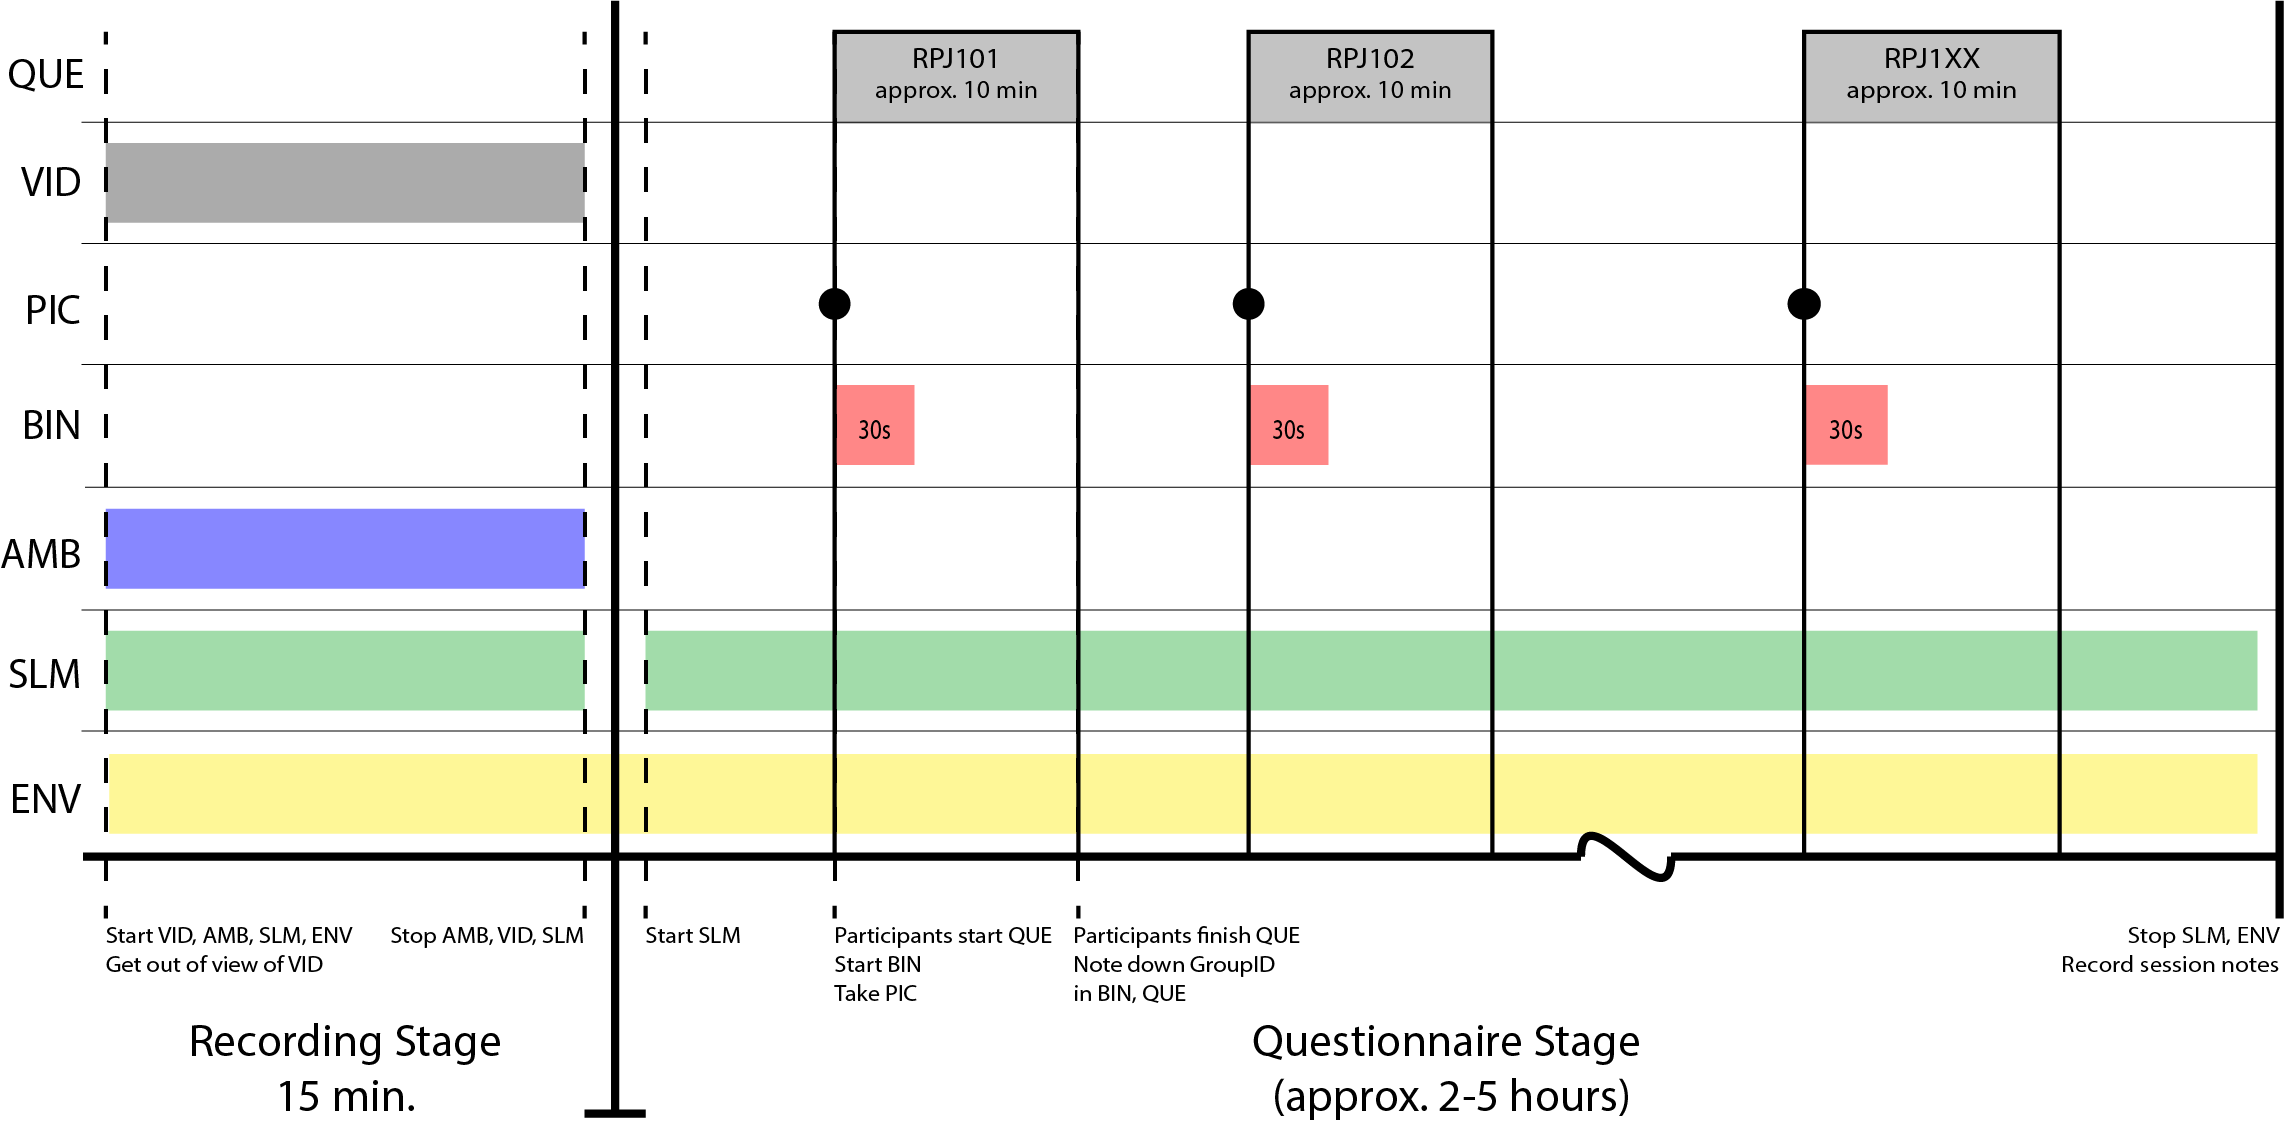
\includegraphics[width=\textwidth]{Figures/Survey-Diagram_V2}
   \caption{Timeline of the on site soundscape protocol. RegentsParkJapan (RPJ) is used as an example. Abbreviations as defined in Table \ref{tab:factors} -- \gls{que}: Questionnaires; \gls{vid}: 360\degree video; \gls{pic}: Site pictures; \gls{bin}: Binaural Recording; \gls{amb}: Ambisonic recording; \gls{slm}: Sound Level Meter (acoustical factors); \gls{env}: Environmental factors.}
   \label{fig:timeline}
 \end{figure}

 \paragraph*{Setup \& Calibration} The equipment should be assembled, checked, and calibrated prior to arriving at the measurement location. Calibrate the equipment according to the manufacturer's instructions. All \gls{slm}s should have built-in methods to calibrate using a standard 94 dB 1 kHz tone calibrator. If a similar method is available for the ambisonic microphone, this should be used. If a built-in method is not available, but a calibrator can be fitted to the microphone capsules, then the ambisonic microphone should be calibrated by recording the 1 kHz signal through the system for each microphone capsule after the gain settings have been finalised on site (see below). If it is not possible to calibrate the ambisonic microphone, then the levels recorded will need to be compared to the levels taken simultaneously with the \gls{slm}. This is why it is crucial to have an appropriate quality, calibrated \gls{slm} included within the same setup as the \gls{amb} recordings.

 \begin{figure}
   \centering
   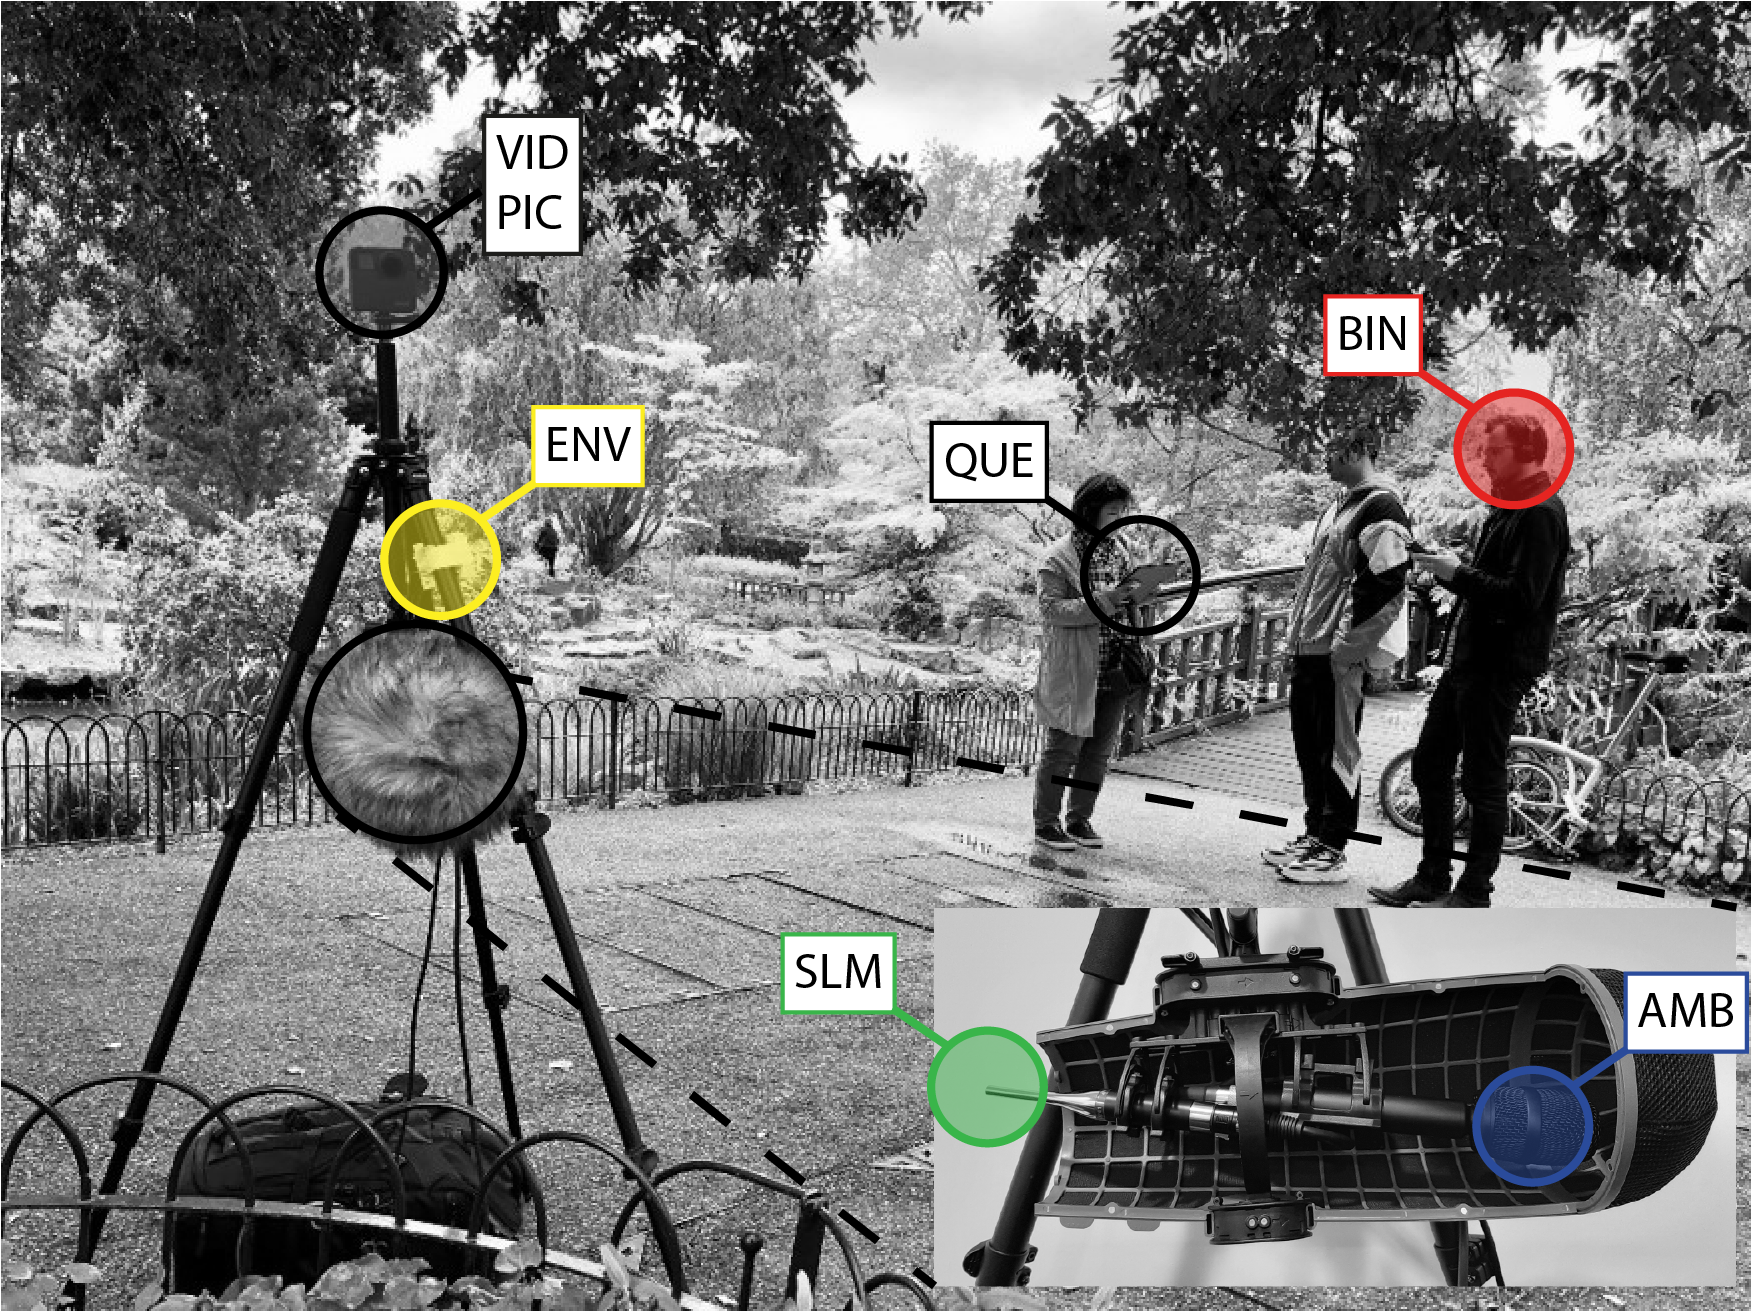
\includegraphics[width=\textwidth]{Figures/RegentsParkSurvey_V2-2}
   \caption{Photo of a full survey carried out in a park in London during the Questionnaire Stage. To the left is the equipment (colour-coded to match Figure \ref{fig:timeline}), with the ambisonic microphone and \gls{slm} microphone in the windscreen, with the 360\degree camera on top of the tripod and to the right are one researcher interacting with the participant while the second researcher conducts the binaural recording. The body of the \gls{slm} and the multi-channel recorder are stored in a bag under the tripod which can contain all of the pieces of equipment for easy transport.}
   \label{fig:survey-pic}
 \end{figure}

 \subsection{Assembling the Equipment}

   \begin{enumerate}
     \item Set up the equipment by prioritising the position of the 360\degree camera and position the lens at the average eye level 160--180 cm, as shown in Figure \ref{fig:survey-pic}.

           It is advisable to test the setup for video stitching issues and reconfigure if needed (e.g. the equipment will be partially visible in the raw video recording, so you need to test if the chosen setup allows for efficient erasing/hiding/patching of the exposed parts in the post-processing). Companies selling 360\degree cameras usually offer free software for basic editing and previewing. It is advisable to position the camera as the highest item in the set to avoid the need for editing both the sky and the ground.
     \item Carefully position the \gls{amb} microphone so its axes are aligned with the axes of the 360\degree camera; the microphone's front (usually marked by the logo) and the camera's front should be looking in the same direction. Many \gls{amb} microphones allow them to be oriented vertically or horizontally (end-fire), this should be noted and adjusted in the relevant software settings.

           This is essential for informed post-processing. It is advisable to position the capsules of the \gls{amb} microphone and the capsule of the \gls{slm} as near to each other as possible, without introducing scattering effects. It can usually be done within the same windshield unit, but it is not essential to do so and depends on the available clamps and stands.
     \item The gain settings for the four ambisonic audio channels should be set to the same level. In some devices (such as the MixPre10), this can be set by locking the channel gain settings to a single channel. Many devices also offer ambisonic plugins which simplify these settings and automatically link the gain settings -- these should be used where available.
     \item Set the \gls{slm} to log sound levels and simultaneously record .wav audio. The recommended logging settings are given in Table \ref{tab:equipment}. The \gls{slm} should be mounted and positioned according to standard guidance for environmental noise measurements, like that given in Section 9 of ISO 1996-2:2017 \cit{ISO1996} or Section 5 of ANSI/ASA S12.9-2013/Part 1 \cit{ANSI}. Generally, the microphone should be a minimum of 1.2m above the ground and a minimum of 1m from any vertical reflecting surfaces.
     \item Attach the environmental meter(s) to the tripod. Care should be taken when positioning the environmental monitor. Most units will include guidance on their use from the manufacturer -- these should be followed where available. Some general items to keep in mind include not accidentally covering air quality sensor holes, not positioning light sensors in the shade of the other equipment, and not positioning temperature sensors in direct sunlight unless this is how they are intended to be positioned.
   \end{enumerate}

 \subsection{Recording Stage}

   The following section prepares step-by-step instructions for conducting the Recording Stage of the on site protocol, as shown in Figure \ref{fig:timeline}.

   \begin{enumerate}
     \item Double check all settings and file save locations on the recording equipment.
     \item Adjust gain settings to ensure there is no clipping. Good practice is to listen for what is expected to be the loudest sound event during the recording period (e.g. sirens) and set the gain such that the level is comfortably under clipping during this event.
     \item Start recording on all devices, including the ambisonic microphone, 360\degree camera, \gls{slm}, and environmental meter.
     \item Stand at the front of the camera/ambisonic microphone and clap. The clap can help synchronise the audio with the video, if necessary, and ensuring you are standing in line with the front of the 360\degree video can help with lining up the directionality of the two, if necessary.
     \item Retreat out of view of the camera, blending into the surrounding crowd, or otherwise make sure not to be obvious to someone watching the video.
     \item Record at least 5 min of consistent and representative audio and video. It is recommended to record for 15 min to give the best chance of being able to extract a solid 5 min of useful video and audio.
     \item Stop recording on all devices and ensure all files are saved properly.
   \end{enumerate}

 \subsection{Questionnaire Stage}

   The following section prepares step-by-step instructions for conducting the in-situ questionnaires and their accompanying reference recordings as part of the Questionnaire Stage. Typically these are performed during the same working session as the Recording Stage, using the same set of equipment. The selection of an appropriate location and setup of the equipment should follow the guidance given in Section \ref{sec:location-selection}, while making sure the location selected is representative of where the respondents will be stopped. Wherever possible, the equipment should be assembled and located so as not to draw the attention of the respondents and particularly to avoid influencing their perception of the space.

   \begin{enumerate}
     \item Double check all settings and file save locations on the recording equipment. If starting this stage immediately after the Recording Stage, make sure to rename or advance the index of on the filenames for the \gls{slm} and \gls{env} meters.
     \item Start recording on the \gls{slm} and \gls{env} meter (or leave running from preceding Recording Stage). These will continue running until the end of the Questionnaire Stage.
     \item Gather the tablets and/or paper questionnaires and prepare to approach potential participants.
     \item Approach participants and ask if they would be willing to take part in a research study. If the participants are in a group, they can participate at the same time, but should each fill out a separate questionnaire. When approaching participants, you should identify yourself as a researcher or student researching urban sound. We %NOTE: May need to change pronouns here
           advise avoiding phrases such as "noise", "noise pollution", "noise disturbance" or other terms which carry a negative connotation. In general, explanations and answers to questions should strive to be as neutral as possible regarding the nature of the soundscape.
     \item Once the participant has consented to participate, hand them the questionnaire or tablet and provide them with basic instructions for answering the questionnaire. Emphasise that they should be responding and assessing the current sound environment, in the current place. Note that this is a common misunderstanding -- many participants assume the questionnaire is focussed on the sound environment at their home, or in the city in general. Where a mix of tablets and paper questionnaires are being used, each group should have at least one participant using a tablet such that start and end times and precise GPS coordinates can be pulled from the accompanying electronic questionnaire. While one researcher is interacting with the participants, the second should arrange the equipment for taking the \gls{bin} recordings and 360\degree photo (\gls{pic}).
     \item Once the participant has started answering the questionnaire, start recording the \gls{bin} audio. If the participants are in a group and all are taking the survey at the same time, only one binaural recording is needed for the whole group. The researcher conducting the recording should strive to keep their head as stationary as possible and to avoid making any extraneous noise.

           Make sure that at least 30s of consistent audio is recorded while the participant is filling in the questionnaire. This should not include talking either from the researcher or the participant. If talking or other intrusive (non-representative) sound occurs, extend the recording period to end up with a solid 30s of good audio. The goal is to capture the sound environment which the participant is exposed to while filling out their questionnaire, but to exclude sounds which the participant is not likely considering as part of their assessment. Most commonly, this would be the researcher talking, or the participant themselves talking. Any other sounds which the participant was "naturally" exposed to should be included.

           When taking the \gls{bin} recording, attempt to orient the head (artificial or researcher wearing a headset) in the same direction as the participants. This is not crucial as it is often impossible to achieve, but it is preferable. Be careful not to move the head during the recording.
     \item Note the GroupID in the metadata for the \gls{bin} recording, or make a manual note of the \gls{bin} recording file name and the GroupID separately.
     \item Take on 360\degree photo (\gls{pic}) with the camera to capture the general setting. This can also be done at regular intervals during the survey session.
     \item When the participant has finished filling in the questionnaire, thank them for their participation and fill in the additional research questions at the end of the questionnaire. These help to both track the data collected and to document the conditions on site. The most important of these are:
           \begin{itemize}
             \item (For paper version) Start and End time. If a Start time was not noted, at minimum, the End Time must be recorded and an average survey duration can be subtracted to estimate the Start Time.
             \item GroupID
             \item SessionID
           \end{itemize}
     \item Repeat steps 4--9 for the remainder of the session, incrementing the GroupID by one with each new group of participants. If there are more than two researchers on site, the additional researchers can stop new groups of participants simultaneously. The researcher operating the \gls{bin} equipment can then shift between the groups once they have finished the 30s recording. This researcher should also have the responsibility of keeping track of the GroupID numbers for each group. Experience has shown this is possible up to about three groups at a time, with four researchers on site.
     \item Once the session is finished, stop the equipment and ensure all files are saved properly.
     \item After each session, make note of the character of the site and the environmental conditions during the survey. This might include, but is not limited to:
           \begin{itemize}
             \item Site typology and intended use (e.g. urban park, transit station, urban square, etc.)
             \item Weather
             \item Crowdedness (i.e. how many people are present in the space)
             \item Dominant sound sources and any key soundmarks
             \item Visual character (e.g. amount of greenness, enclosed vs. open, etc.)
           \end{itemize}
   \end{enumerate}

\section{Lessons from International Data Collection}

 As this protocol has already been implemented by several research groups across four countries, it has undergone a rigorous testing and development process. Throughout this process, adjustments have been made which resulted in the final protocol presented here. However, no process is perfect or applicable in all situations. As such, after consultation with the research groups involved, we have compiled the most common feedback and guidance to keep in mind when implementing this protocol.

 \subsection{Sampling}

   The research groups were instructed to try keeping the structure of respondents well-balanced. This often led to longer times and larger sample sizes required as most comments from five research groups addressed age and type of location as the most influential factors for participant sampling. However, while some reported higher response rates from younger (student) members of the public, the others reported higher response rates in case of older highly-educated people. A common observation was that public parks are the locations with the highest response rates, most likely due to a high number of people taking part in activities that allow enough time to take part in a survey. The type of space was also reflected in the sense of privacy. In locations that were more public, people in groups were more likely to take part in the survey, while in the more private locations it was the opposite. Amongst other comments, whether a participant was a tourist or a local also had an influence on the response rate. Tourists seemed more likely to participate in the survey.

   Several groups reported excessive heat and cold to be negatively affecting the response rates. One research groups, which conducted the survey also in a residential area, distinguished privacy/ownership of the survey site as a major factor.

 \subsection{Data Collection}

   A group of three researchers seems to be the minimum number needed to conduct the survey, as observed by the partner research groups. A group of nine researchers on site proved to be the most effective number. The time needed to complete the survey varied greatly depending on the location.

   Although the questions are written in a manner that emphasises the focus on the actual acoustic environment perceived at the moment, additional care should be made to ensure a proper understanding of that concept while approaching the participants. Researchers' comments are invaluable here to keep track of the outliers if a researcher feels similar issues or other factors (i.e. wearing headphones) lead to collecting invalid or misleading data.

 \subsection{Equipment}

   Some partners had previous experience in soundscape research, but for all this was the first study that featured surveying a large number of public participants around a single measurement point. All the research groups found it very important to delegate one researcher or technician to care exclusively about the equipment and the quality of the recordings.

   The intention of the recording stage is to record a first-person experience most representative of the location. Therefore, the researchers are instructed to 'make themselves invisible' in the recording. However, at some locations, various research groups decided to put out a sign asking members of the public asking members of the public not to touch or come near the measurement point as they experienced passers-by touching the windshield out of curiosity.

   The equipment setup has been designed to be as compact and unobtrusive as possible so as to limit any intrusion on the participant's experience of the space. From our experience, most participants do not end up with the equipment within their field of view during the questionnaire and often do not notice the presence of the stationary equipment. In some locations, this is not possible and participants may comment on its presence; however, over the thousands of surveys collected, only a small number of respondents have commented on the equipment as noticeably impacting their experience.

 \subsection{Translation}

   Regarding the onsite soundscape survey, the translation of the questionnaires (and in particular the perceptual adjectives used for the soundscape appraisal) is a key point to consider when using the protocol in regions where English is not the local language. Indeed, while the ISO/TS 12913-2:2018 document from which the soundscape-related questions of this protocol are derived aims at providing standardised scales, it does not provide official translations in languages other than English. Some perceptual constructs are difficult to render in different languages and people might assign different meanings to them (e.g. \cit{51-54}). For this reason, in the soundscape research community, there is a growing interest in testing and validating reliable translation of the ISO soundscape adjectives \cit{Aletta SATP}, which will hopefully lead to a wide-spread use of this soundscape tool. It is expected that these validated translations could simply be substituted for their English counterparts in this protocol, when they become available.